\chapter{Proposed Design}
\label{chap:design}

The design in this report is based upon a design\cite{1584083} for a programmable memory BIST with auxiliary memory for background patterns.  This design (proposed design) will modify the programmable memory BIST design (base design) by introducing a pattern generator to dynamically generate the NPSF Type-1 neighborhood patterns.  It will also replace the address counter with a programmable address generator to allow more flexibility in testing specific address sequences.  Section \ref{sect:bg-blocks} describes the base design's major blocks in more detail.  Details of the proposed design's modifications follow in section \ref{sect:bg-modifications}.

\section{PMBIST Hardware Blocks}
\label{sect:bg-blocks}
The proposed design is comprised of five major blocks: the scan and instruction register; the cycle controller; the address generator block; the data generator and compare block; and the operation control block;.  The major blocks and their connections are illustrated in Fig. \ref{fig:pmbistall} and the following sections descibe the blocks in more detail.

\begin{figure}[h]
  \centering
  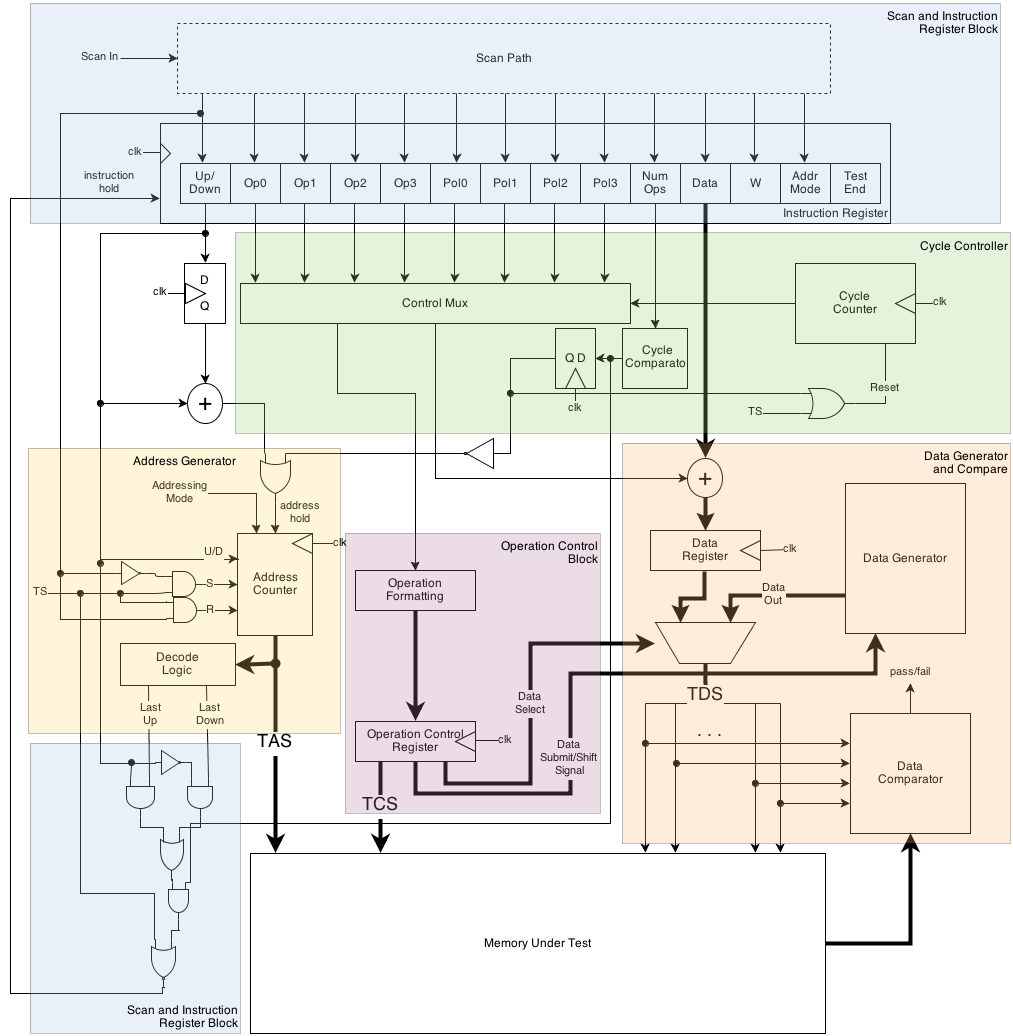
\includegraphics[scale=0.4]{pmbistall}
  \caption{Major Block of the PMBIST Design}
  \label{fig:pmbistall}
\end{figure}

\subsection{Cycle Controller}
The cycle controller determines which march operation should execute on the current address.  When all march operations have completed on the current address, the cycle controller generates a signal that allows the address counter to move to the next test address.  The cycle controller then resets the march operation pointer to the first operation for the next address.   

\subsubsection{Control Mux}
The control mux receives all the operation and polarity signals from the instruction register.  Using the cycle counter's output as the mux control signal, the control mux selects the operation and polarity signal corresponding to the current cycle and outputs them to the operation formatting block and control register.  

\subsubsection{Cycle Counter}
The cycle counter increments the count for the march operation to execute.  The output of the cycle counter corresponds to the active march operation.  The cycle counter is incremented by the clock signal and can be reset by a TS signal or when the current march sequence has completed for the current memory address. 

\subsubsection{Cycle Comparison}
The cycle comparison unit compares the current cycle to the NO field of the instruction register.  When the cycle counter matches the NO field, the comparison block generates an active high signal that is stored in the cycle controller's local flip-flop.  The signal is also sent to the instruction register hold logic block.  

\subsection{Address Generation}
The memory address to test and memory control signals are generated by the address and operation block.  The address decode block is used to generate the instruction register hold signal.  The hold signal maintains the instruction register's data until the current march sequence has completed for all memory address.  

\subsubsection{Address Counter}
The address counter indicates the memory address to test.  The direction of the address order can be programmed to increment or decrement through memory.  The order of addresses is also programmable: linear up/down, pseudo-random sequence using LFSR, address complement, Gray coding, and 2\textsuperscript{i} counting methods.
 
\subsubsection{Address Decode Logic}
The address decode logic block determines if the address generated by the address counter is the last up (LU) or last down (LD) memory address for the current march sequence.  The decode logic uses the signals from the address programmer block to determine whether the sequence direction is up or down.   

\subsection{Operation Control Block}
In some designs, the memory algorithm operation signals from the instruction register do not necessarily need to match the memory's control signals.  The operation formatting block can be used to translate the instruction register's operation code to the memory controller's signals such as write/read, enable and reset.

\subsubsection{Operation Formatting}
The Operation Formatting block converts the memory algorithm operation signal to explicit memory control signals such as read/write, enable and reset.  The output of this block passes to the control register.

\subsubsection{Operation Control Register}
The control register interprets the operation formatted instruction and sends any internal control signal to other blocks of the PMBIST.  In particular, this block sends the data mux select signal and controls the sequencing of the data generator.  It also writes the memory control signals to the TCS bus.  

\subsection{Data Generator and Compare}
Data can come from the instruction register or the data generator.  A mux select signal is generated based on the current operation.  For user data patterns, the data from the instruction register is selected and written to memory.  For NPSF patterns, the data generator outputs the word to be written to memory.  The comparator checks if the data read from memory matches what is expected and generates the pass/fail signal.

\subsubsection{Data Generator}
\begin{figure}[h!]
  \centering
  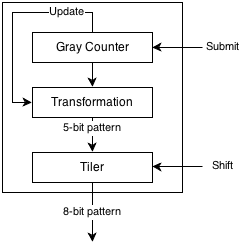
\includegraphics[scale=0.5]{datagen}
  \caption{Data Generator Block Diagram}
  \label{fig:datagen}
\end{figure}
The data generator block design is shown in \ref{fig:datagen}.  The gray counter is a 5-bit counter that generates gray code and repeats after 32 iterations.  The gray code is passed to the transform block which converts the code to a Eulerian Sequence.  A detailed description of the Euler Sequence can be found in \cite{1675556}.  Essentially, a 5-bit Euler Sequence used as the Type-1 NPSF background will transition through all the possible read and write combinations that could occur.  This requires 161 different sequences which can be broken into five groupings as shown in \ref{tab:euler}.  Except for the first column, each column is generated by a one-bit right shift and rotate followed by inverting the most and least significant bits \cite{00957583}.

\begin{table}[h]
  \caption{Partial 5-bit Euler Sequence}
  \centering
  \begin{tabular}{c c c c c c}
  \hline\hline
  Iteration    & Gray (E[0]) & E[1]  & E[2]  & E[3]  & E[4]  \\
  X0  & 00000 & 10001 & 01001 & 00101 & 00011 \\
  X1  & 00001 & 00001 & 00001 & 00001 & 00001 \\
  X2  & 00011 & 00000 & 10001 & 01001 & 00101 \\
  ......             & ...   & ...   & ...   & ...   & ...   \\
  X29 & 10011 & 01000 & 10101 & 01011 & 00100 \\
  X30 & 10001 & 01001 & 00101 & 00011 & 00000 \\
  X31 & 10000 & 11001 & 01101 & 00111 & 00010 \\ [0.5ex]
  \end{tabular}
  \label{tab:euler}
\end{table}

The transformation block provides the 5-bit Euler Sequence to be used as the NPSF background.  To write this value to memory using the Type-1 tiling method, the sequence must be spread over the adjacent rows to create the correct tiling background as shown in \ref{fig:tiling}.  

\begin{figure}[h!]
  \centering
  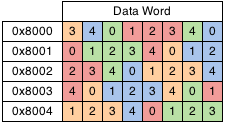
\includegraphics[scale=0.5]{type1tiling}
  \caption[Type-1 Neighborhood Tiling Method for Design]{Type-1 Neighborhood Tiling Method for Design}  
   Each 5-bit color block represents one Type-1 neighborhood.
  \label{fig:tiling}
\end{figure}

\subsubsection{Data Comparator}
Each read march element is checked with the data comparator.  The comparator accepts as inputs the TDS bus and the output of the MUT.  If the MUT output matches the TDS value, a pass signal is generated.  If there is any discrepancy, the fail signal is generated.  

\subsubsection{Polarity and Data Register}
The polarity signal from the current march operation is used to invert the data.  If the polarity signal is false (0), the data is unmodified and stored to the data register.  If the polarity signal is true (1), the data is inverted, then stored in the data register.  

\subsection{External Connections}
Integration with the MUT and scan-path requires a few external connections.  The scan-path writes data to the instruction register for the test.  The MUT receives address, data and control signals from the memory BIST.

\subsubsection{Scan-Path Connection}
The scan-path receives data serially for the memory BIST.  The scan-path signals correspond to the instruction register fields.  When the scan-in data has been clocked into place, the instruction register will latch the data and begin its test.  

\subsubsection{Memory Under Test Connections}
The MUT connects to the MBIST through the test buses.  The connections provides the data, control signals and address to the memory and are connected to the memory input pins.  

\paragraph{Test Address Signals}
The test address signals (TAS) compose the memory address currently on interest to the test.  They can point to the read address for a comparison or check or the write address to store new data.

\paragraph{Test Control Signals}
The test control signals (TCS) are generated from the instruction register's operation field.  The signals are formatted to work with the MUT.  The opcode is translated to the memory control signals such as read/write, reset and enable.  

\paragraph{Test Data Signals}
The test data signals (TDS) contain the data to be stored in memory.  These signals are connected to the MUT's data input pins and the data comparator's input pins.  They are driven from the data register.  When an auxiliary memory is used, the data pins are driven from the outputs of the auxiliary memory.


\section{Modifications to Programmable MBIST}
\label{sect:bg-modifications}
These modifications were made to the design.

\subsection{Address Generator Expansion}
The address generator originally supported linear and pseudo-random address counting methods.  The design in this report will add Gray code, address complement and 2\textsuperscript{i} counting methods.

\subsection{Programmable Address Generator}
The original design did not make use of the address mode field and left it to the designer to decide on whether to implement the psuedo-random or linear counting methods.  The only programmability for address was the direction which was set using the up/down field.  This report adds the ability to select which address generation pattern to use.  The instruction register was expanded with new fields for address generation modes to allow programmability, and the instruction field is decoded within the BIST to select the address counting method.

\begin{table}[hbt]
  \caption{PMBIST Address Modes}
  \centering
 \begin{tabular}{|p{1in}|p{0.75in}|p{3in}|}
  \hline
  Name & Op Code (binary) & Description \\ [0.5ex]
  \hline\hline
  Linear              & 0000 & Standard numerical sequence  \\ 
  \hline
  Pseudo-Random       & 0001 & Repeatable random sequence \\ 
  \hline
  Address \ Complement  & 0010 & Progresses linearly on even steps and inverts all bits on odd steps.\\ 
  \hline
  \textit{Reserved}            & 01XX & Available for additional addressing modes \\ 
  \hline
  Gray Coding         & 0011 & Changes only one bit per address transistion \\ 
  \hline
  2\textsuperscript{\textit{i}}& 1[j\textsubscript{2:0}] & Generates all address pairs with a \textit{Hamming} distance of 1.  2\textsuperscript{\textit{i}} = \textit{j}\textsubscript{2:0} where \textit{i} is the address bit that determines address-pair for \textit{Hamming} distance. \\ 
  \hline
 \end{tabular}
\label{tab:addrmode}
\end{table}

\subsection{Dynamic Background Pattern Generation}
The auxiliary memory is used to store NPSF background patterns in the base design.  To reduce the area required by this design, the auxiliary memory is replaced by a dynamic background pattern generator.  The generator creates the Type-1 neighborhood pattern and translates it to an 8-bit value that can be written sequentially to memory to create the background pattern.




